
\begin{centering}
\def\s{2} % F_g

\begin{tikzpicture}[>=stealth,tdplot_main_coords]
    	\coordinate (O) at (0,0,0);
   	\coordinate (A) at (0,\s,0);
   	\coordinate (B) at ({sqrt(3)/2*\s},{\s/2},0);
	\coordinate (C) at ({sqrt(3)/6*\s},{\s/2},{sqrt(6)/3*\s});
    
    	%\draw[->] (O) -- (6,0,0);
    	%\draw[->] (O) -- (0,6,0);
    	%\draw[->] (O) -- (0,0,6);
    
    	
    	\draw[blue,fill=yellow!50] (O) -- (A) -- (B) -- cycle;
    	\draw[blue,fill=red!20] (O) -- (A) -- (C) -- cycle;
    	
    	\draw[blue,fill=green!10] (A) -- (B) -- (C) -- cycle;
    	
    	\draw[fill=red]  ($(A)!0.5!(B) $)  circle [radius=0.075cm];
    	\draw[fill=blue]  ($(A)!0.5!(C) $)  circle [radius=0.075cm];
    	\draw[fill=red]  ($(O)!0.5!(A) $)  circle [radius=0.075cm];
    	
    	\draw[fill=red] (A) circle [radius=0.1cm];
    	\draw[blue,fill=blue!10,opacity=0.6] (O) -- (B) -- (C) -- cycle;

	\draw[fill=red] (O) circle [radius=0.1cm];
    	
    	\draw[fill=red] (B) circle [radius=0.1cm];
    	\draw[fill=green] (C) circle [radius=0.1cm];
    	
    	
    	\draw[fill=red]  ($(O)!0.5!(B) $)  circle [radius=0.075cm];
    	\draw[fill=blue]  ($(O)!0.5!(C) $)  circle [radius=0.075cm];
    	
    	\draw[red, thick] (O) -- (B) -- (A) -- cycle;
    	\draw[blue, thick] ($(A)!0.5!(C) $) -- ($(C)!0.5!(B) $) --($(C)!0.5!(O) $) -- cycle;
    	
    	
    	
    	\draw[fill=blue]  ($(C)!0.5!(B) $)  circle [radius=0.075cm];
    	
\end{tikzpicture}
\enspace
\huge{$\Rightarrow$}
\enspace

\begin{tikzpicture}
	\draw[fill=green] (0,0) circle [radius=0.1cm];
\end{tikzpicture}
\enspace
\huge{+}
\enspace
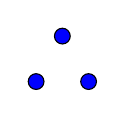
\begin{tikzpicture}
	\draw[fill=blue] (0,0) circle [radius=0.1cm];
	\draw[fill=blue] ({1*2/3},0) circle [radius=0.1cm];
	\draw[fill=blue] ({1/2*2/3},{sqrt(3)/2*2/3}) circle [radius=0.1cm];
\end{tikzpicture}
\enspace
\huge{+}
\enspace
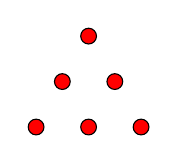
\begin{tikzpicture}
	\draw[fill=red] (0,0) circle [radius=0.1cm];
	\draw[fill=red] (2/3,0) circle [radius=0.1cm];
	\draw[fill=red] ({1/2*2/3},{sqrt(3)/2*2/3}) circle [radius=0.1cm];
	\draw[fill=red] ({-1/2*2/3},{-sqrt(3)/2*2/3}) circle [radius=0.1cm];
	\draw[fill=red] ({1/3},{-sqrt(3)/3}) circle [radius=0.1cm];
	\draw[fill=red] ({3/3},{-sqrt(3)/3}) circle [radius=0.1cm];
\end{tikzpicture}
\end{centering}